\documentclass[25pt,a0paper,portrait]{tikzposter}
\usepackage{graphicx}
\usepackage{booktabs}
\usepackage{array}
\usepackage{lmodern}
\usetheme{Board}

% Spain's flag red
\definecolor{spainred}{RGB}{196,30,58}
\definecolor{spainlight}{RGB}{250,230,230}

\colorlet{titlebgcolor}{spainred}
\colorlet{titlefgcolor}{white}
\colorlet{blocktitlebgcolor}{spainred}
\colorlet{blocktitlefgcolor}{white}
\colorlet{blockbodybgcolor}{white}

\title{\textbf{COVID-19 in Spain} \quad {\normalsize a data story, with Poland as benchmark}}
\author{DAV Project 2026 \textbullet\ University of Warsaw}
\institute{Data sources: Our World in Data \textbullet\ ISCIII (Spanish Ministry of Health)
  \textbullet\ Oxford OxCGRT \textbullet\ Google Community Mobility \textbullet\ Eurostat \textbullet\ INE}

\begin{document}
\maketitle

% ── Full-width key-numbers banner ───────────────────────────────────────────
\block[bodyinnersep=1.2em]{Spain in five numbers}{
  \centering
  \renewcommand{\arraystretch}{1.4}
  \begin{tabular}{>{\centering\arraybackslash}p{0.18\linewidth}
                  >{\centering\arraybackslash}p{0.18\linewidth}
                  >{\centering\arraybackslash}p{0.18\linewidth}
                  >{\centering\arraybackslash}p{0.18\linewidth}
                  >{\centering\arraybackslash}p{0.18\linewidth}}
    \textbf{\Huge{>120{,}000}} &
    \textbf{\Huge{342}} &
    \textbf{\Huge{66\%}} &
    \textbf{\Huge{16.5\%}} &
    \textbf{\Huge{12.5\%}} \\
    confirmed COVID-19 deaths (2020--2024) &
    deaths per 100{,}000 population &
    fewer international tourist arrivals in 2020 &
    peak unemployment rate (Q3 2020) &
    peak test-positivity, far above WHO 5\% threshold \\
  \end{tabular}
}

% ── Context block (full width, text-heavy) ──────────────────────────────────
\block{What this poster shows --- and why Spain?}{
  \large
  Spain was one of the European countries hit earliest and hardest by SARS-CoV-2.
  Madrid recorded community transmission already in late February 2020, and the
  national State of Alarm (14 March 2020) imposed one of the strictest lockdowns
  on the continent. With a tourism-dependent economy ($\sim$12\% of GDP) and an
  ageing population (median age 44), Spain combines an unusually severe
  epidemiological shock with an unusually severe \emph{economic} shock --- which
  is why we chose it. Throughout the poster we benchmark Spain against
  \textbf{Poland}, a country with a similar population size but a very different
  pandemic timeline, demographic profile and policy response.

  \textbf{Definitions used.}
  \emph{Cases} = laboratory-confirmed SARS-CoV-2 infections reported by ISCIII /
  OWID. \emph{Excess mortality} = observed deaths minus the 2015--2019 baseline
  for the same calendar week (Eurostat). \emph{Stringency index} = 0--100 score
  of containment policies (Oxford OxCGRT). \emph{CFR} = case-fatality rate =
  deaths / confirmed cases (a biased estimator, see Wave Analysis). All
  population-adjusted figures use 2020 INE / Eurostat populations.
}

\begin{columns}

% ── LEFT COLUMN ─────────────────────────────────────────────────────────────
\column{0.33}

\block{The epidemic curve}{
\begin{tikzfigure}[Daily new cases per 100k inhabitants, Spain vs Poland.
  Five clear waves: the catastrophic first wave (Mar--May 2020, mostly
  invisible in confirmed cases because testing was unavailable), the summer
  2020 resurgence, alpha (winter 20/21), delta (summer 21) and omicron (winter
  21/22). After 2022, reporting changes flatten the curve.]
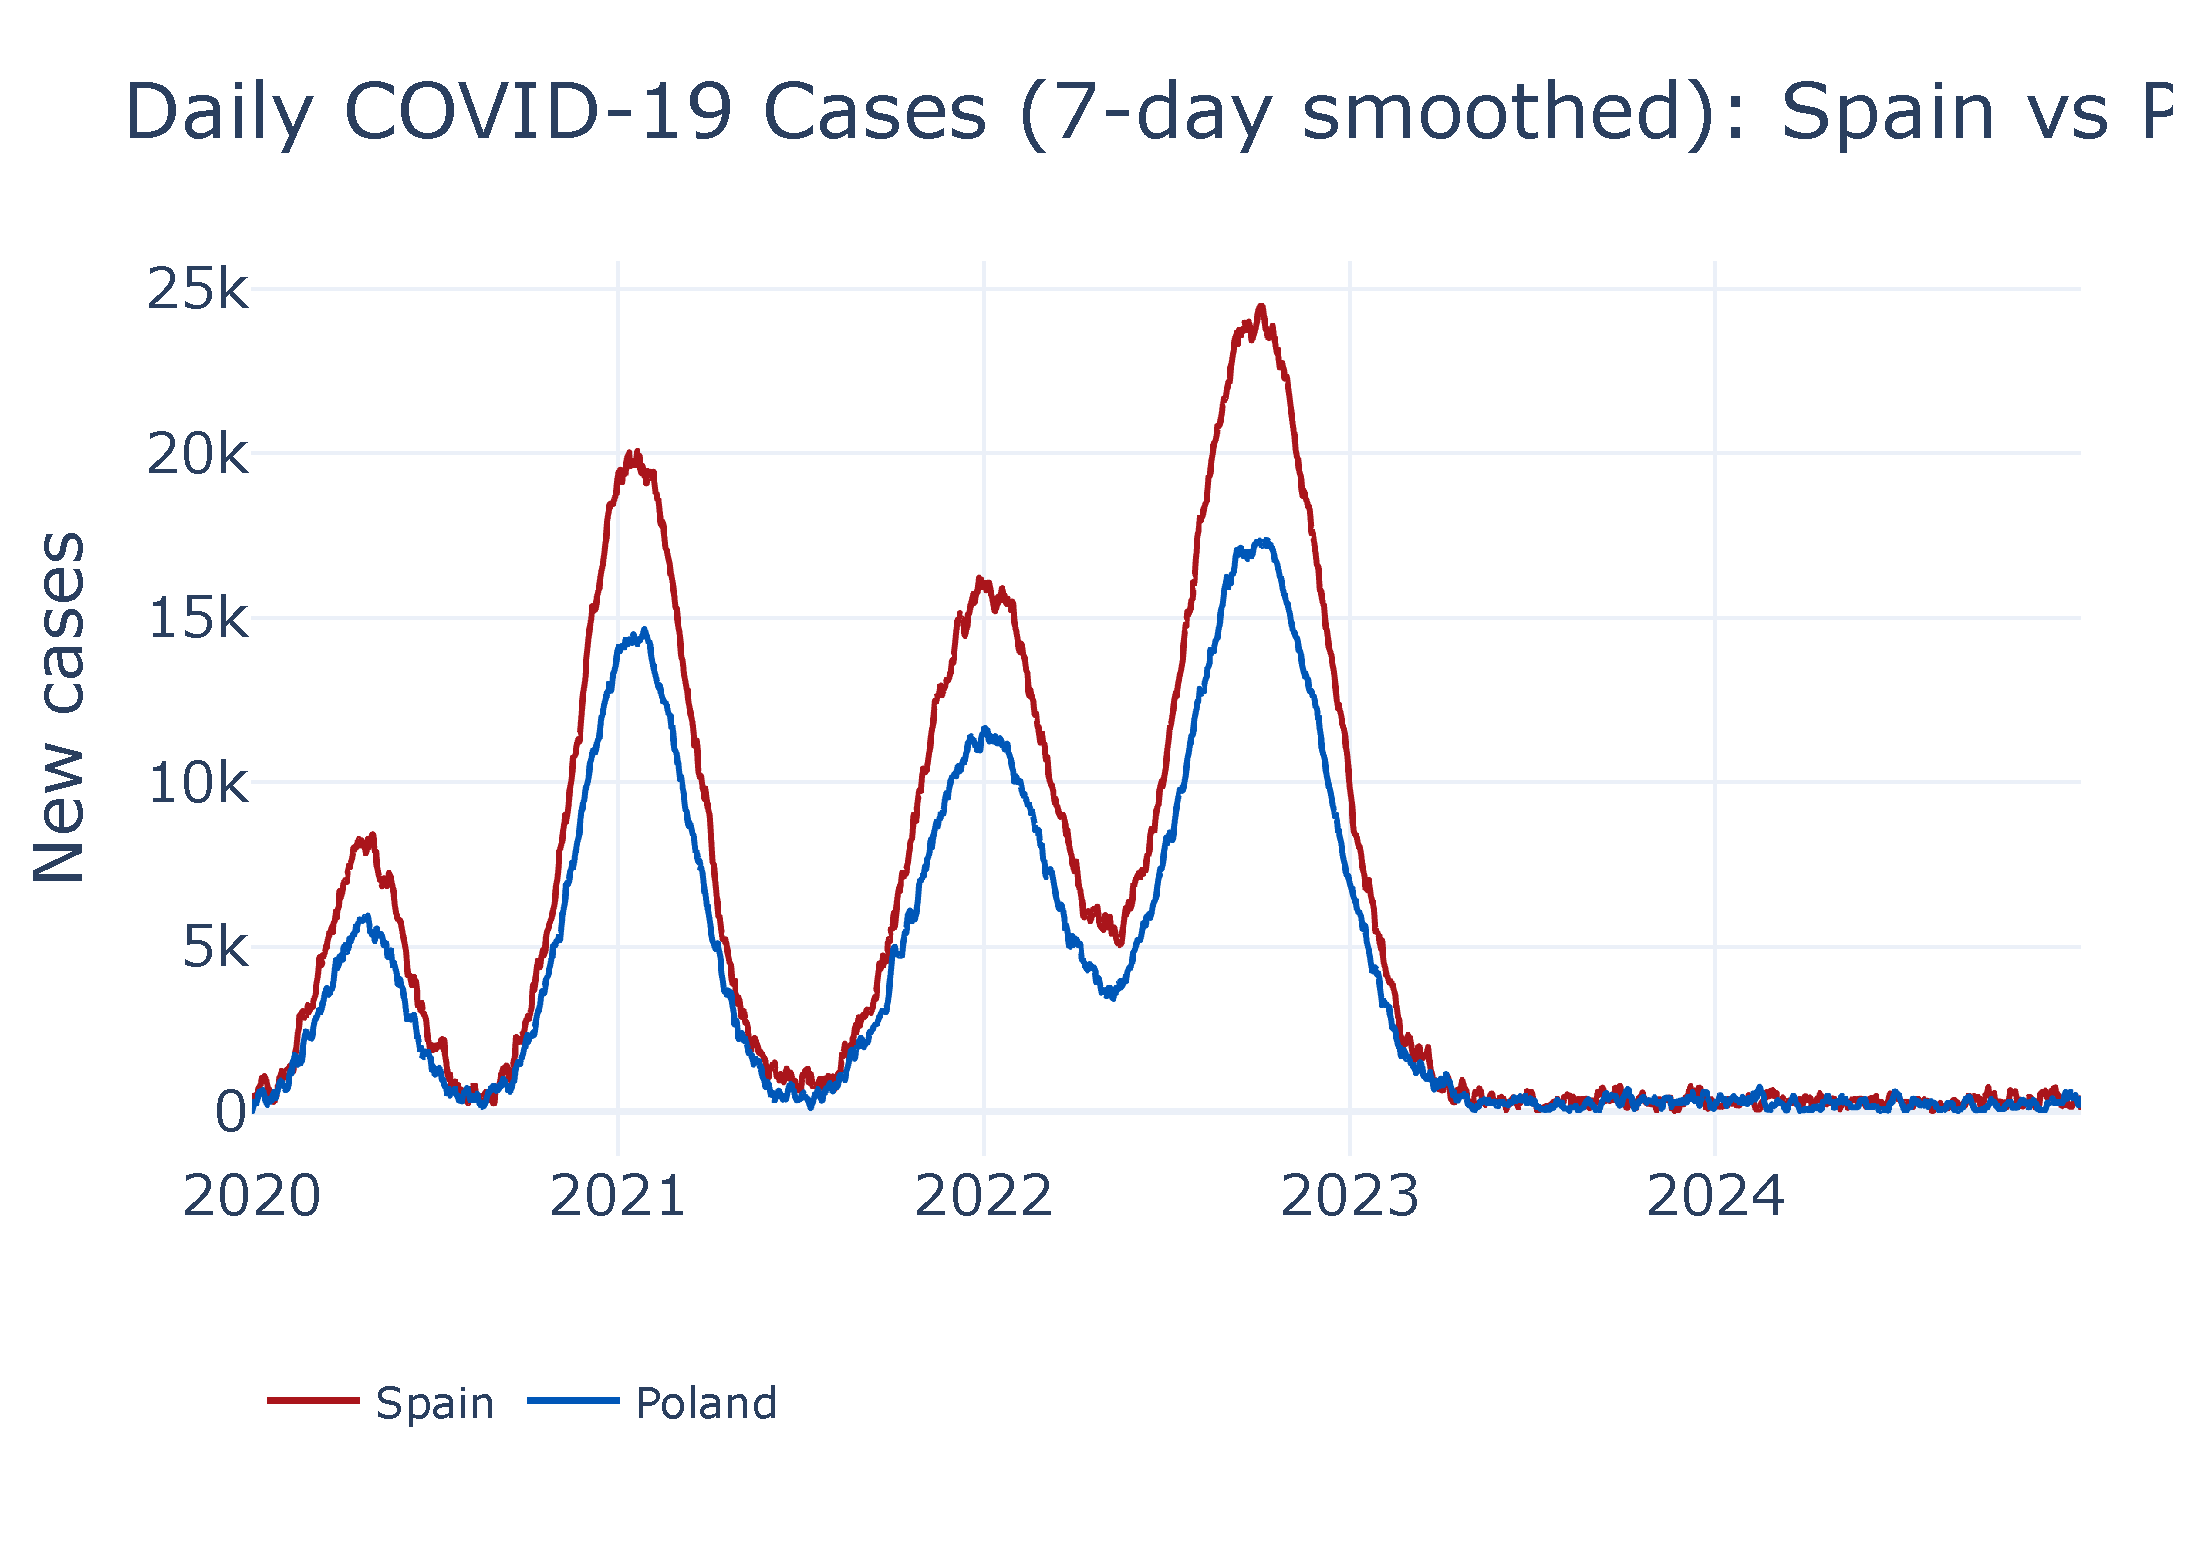
\includegraphics[width=0.95\linewidth]{../figures/static/01_cases_timeline.pdf}
\end{tikzfigure}

\vspace{0.5em}
\large
The first wave dwarfs everything else in mortality but is barely visible in
\emph{confirmed} cases --- a measurement artefact, not a real low. Excess
mortality (next block) corrects for this and tells the real story.
}

\block{The true toll: excess mortality}{
\begin{tikzfigure}[Weekly excess deaths over the 2015--2019 baseline (Eurostat).
  The spring-2020 peak in Spain is one of the largest ever recorded in a
  European country in peacetime. Subsequent waves are visible but progressively
  smaller --- vaccination and acquired immunity blunted later peaks.]
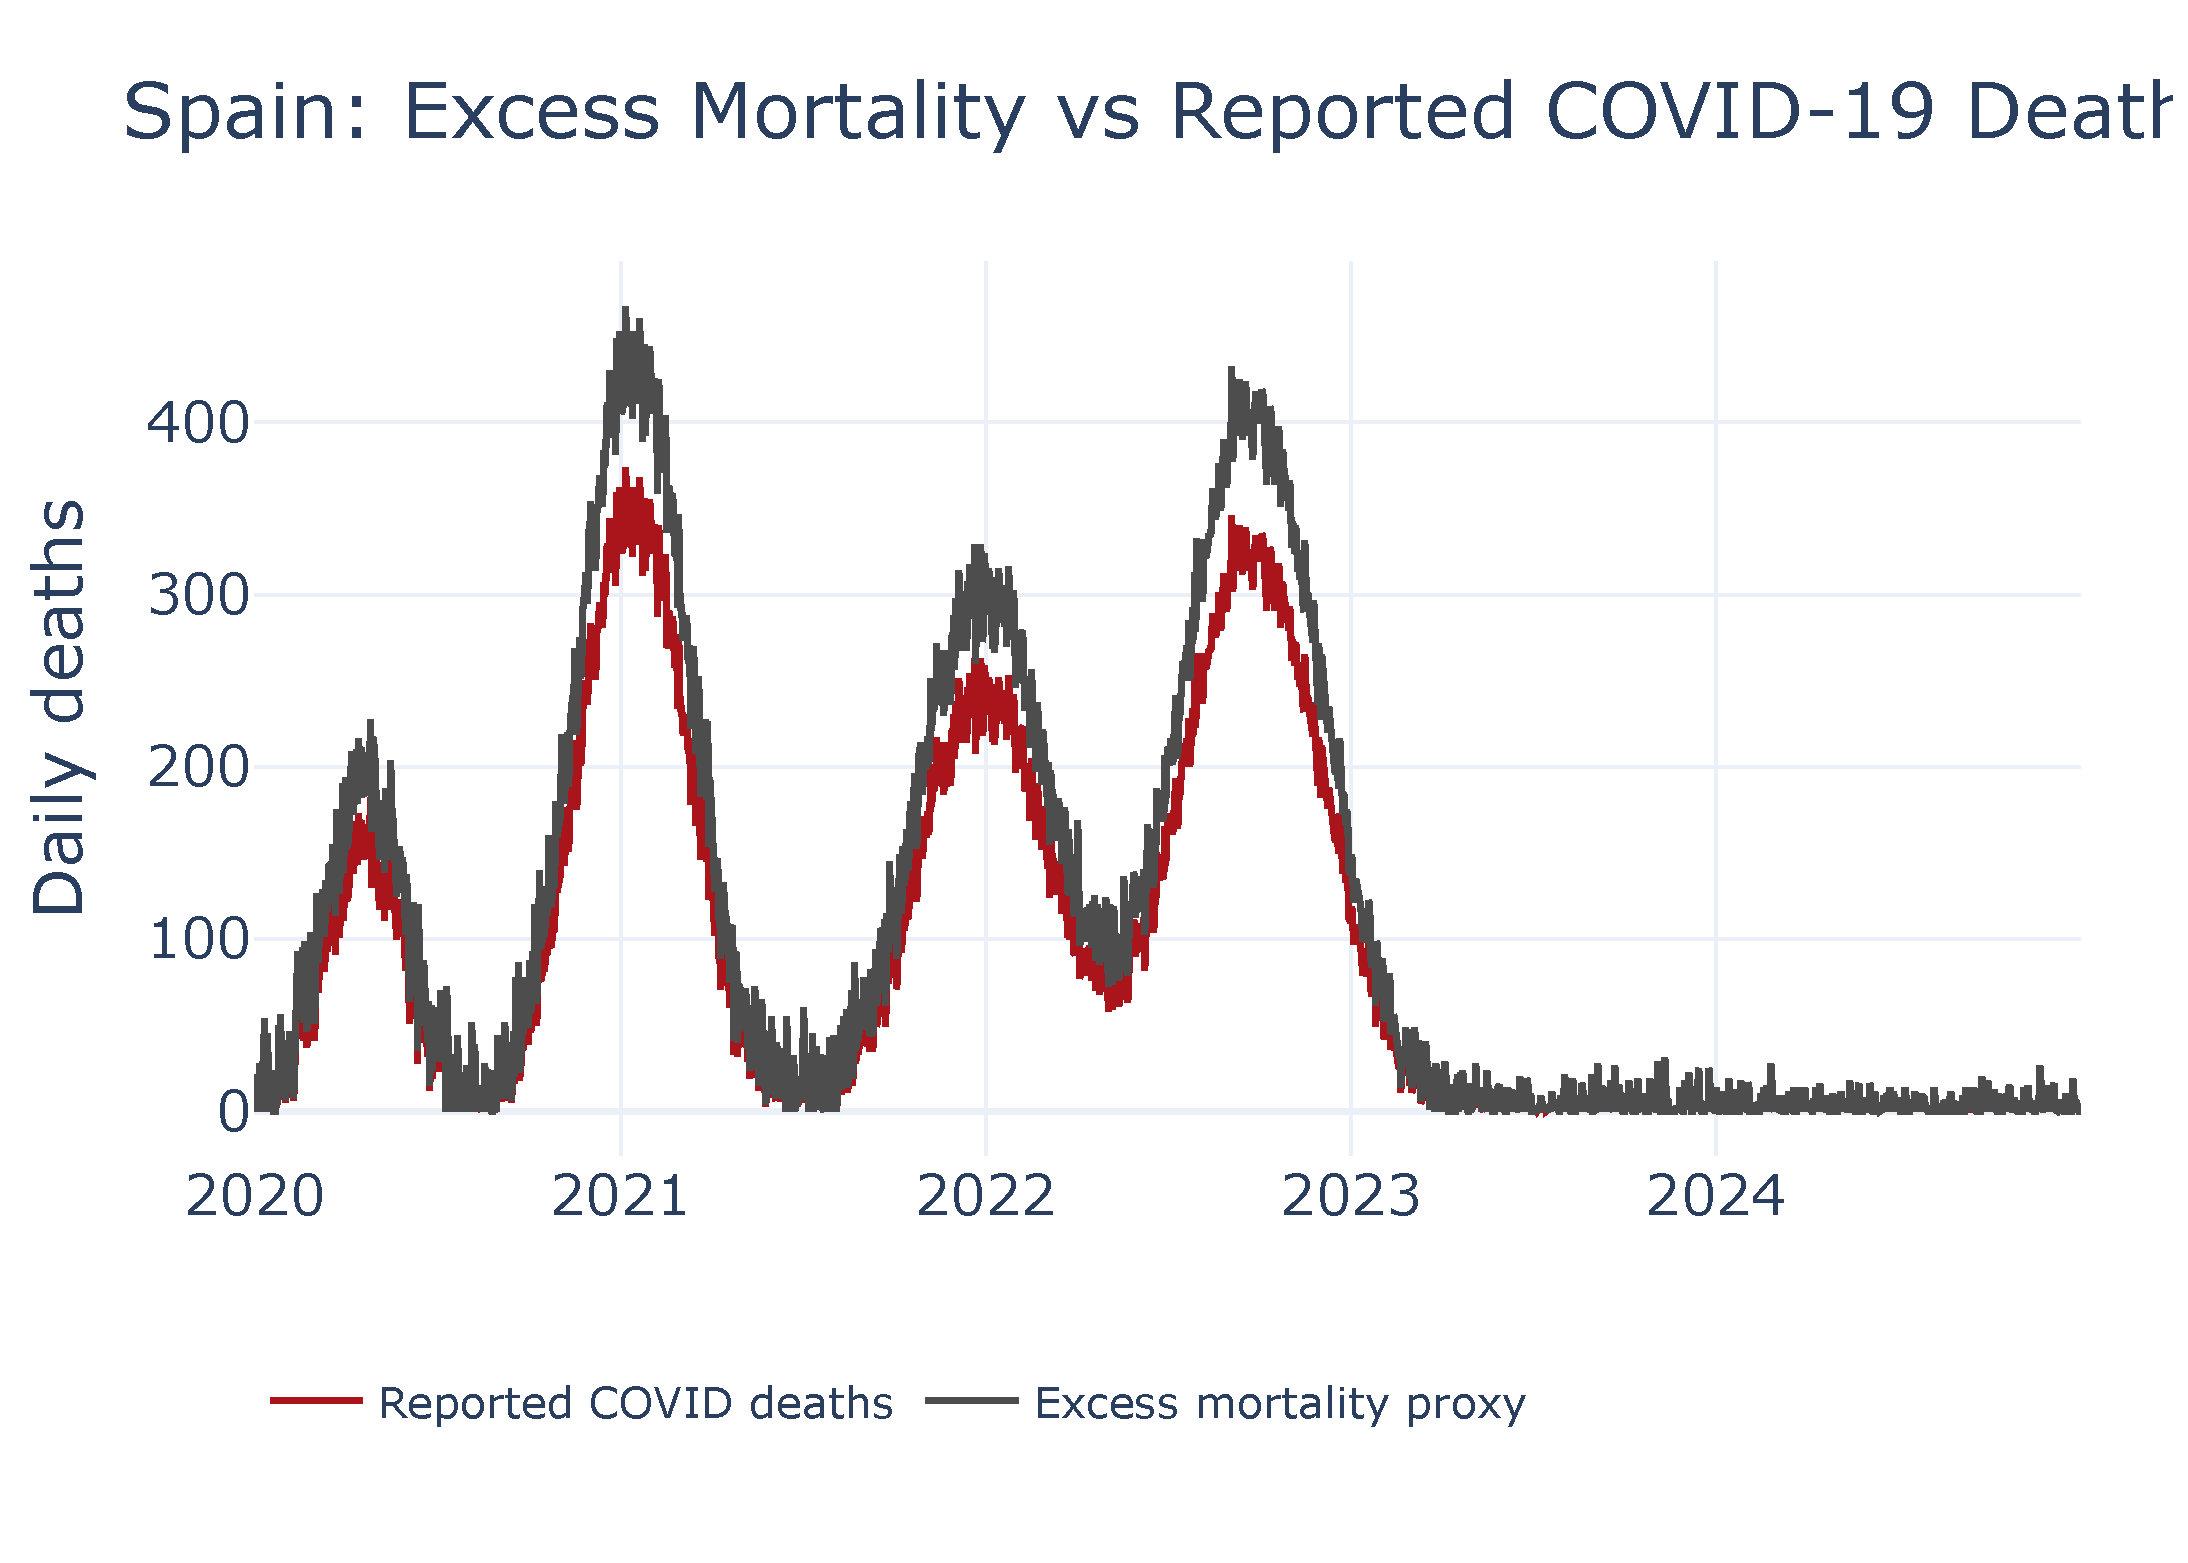
\includegraphics[width=0.95\linewidth]{../figures/static/05_excess_mortality.pdf}
\end{tikzfigure}

\vspace{0.5em}
\large
\textbf{Why this matters.} Confirmed-death counts depend on testing capacity
and definitions. Excess mortality does not --- making it the most reliable
single indicator of pandemic severity.
}

% ── MIDDLE COLUMN ───────────────────────────────────────────────────────────
\column{0.34}

\block{Where and who: the regional and demographic story}{
\begin{tikzfigure}[Cumulative cases per 100k by wave across Spain's 17
  autonomous communities. Madrid leads the first wave; later waves spread more
  uniformly, with inland communities (Aragón, Castilla y León) bearing higher
  per-capita burden than the islands.]
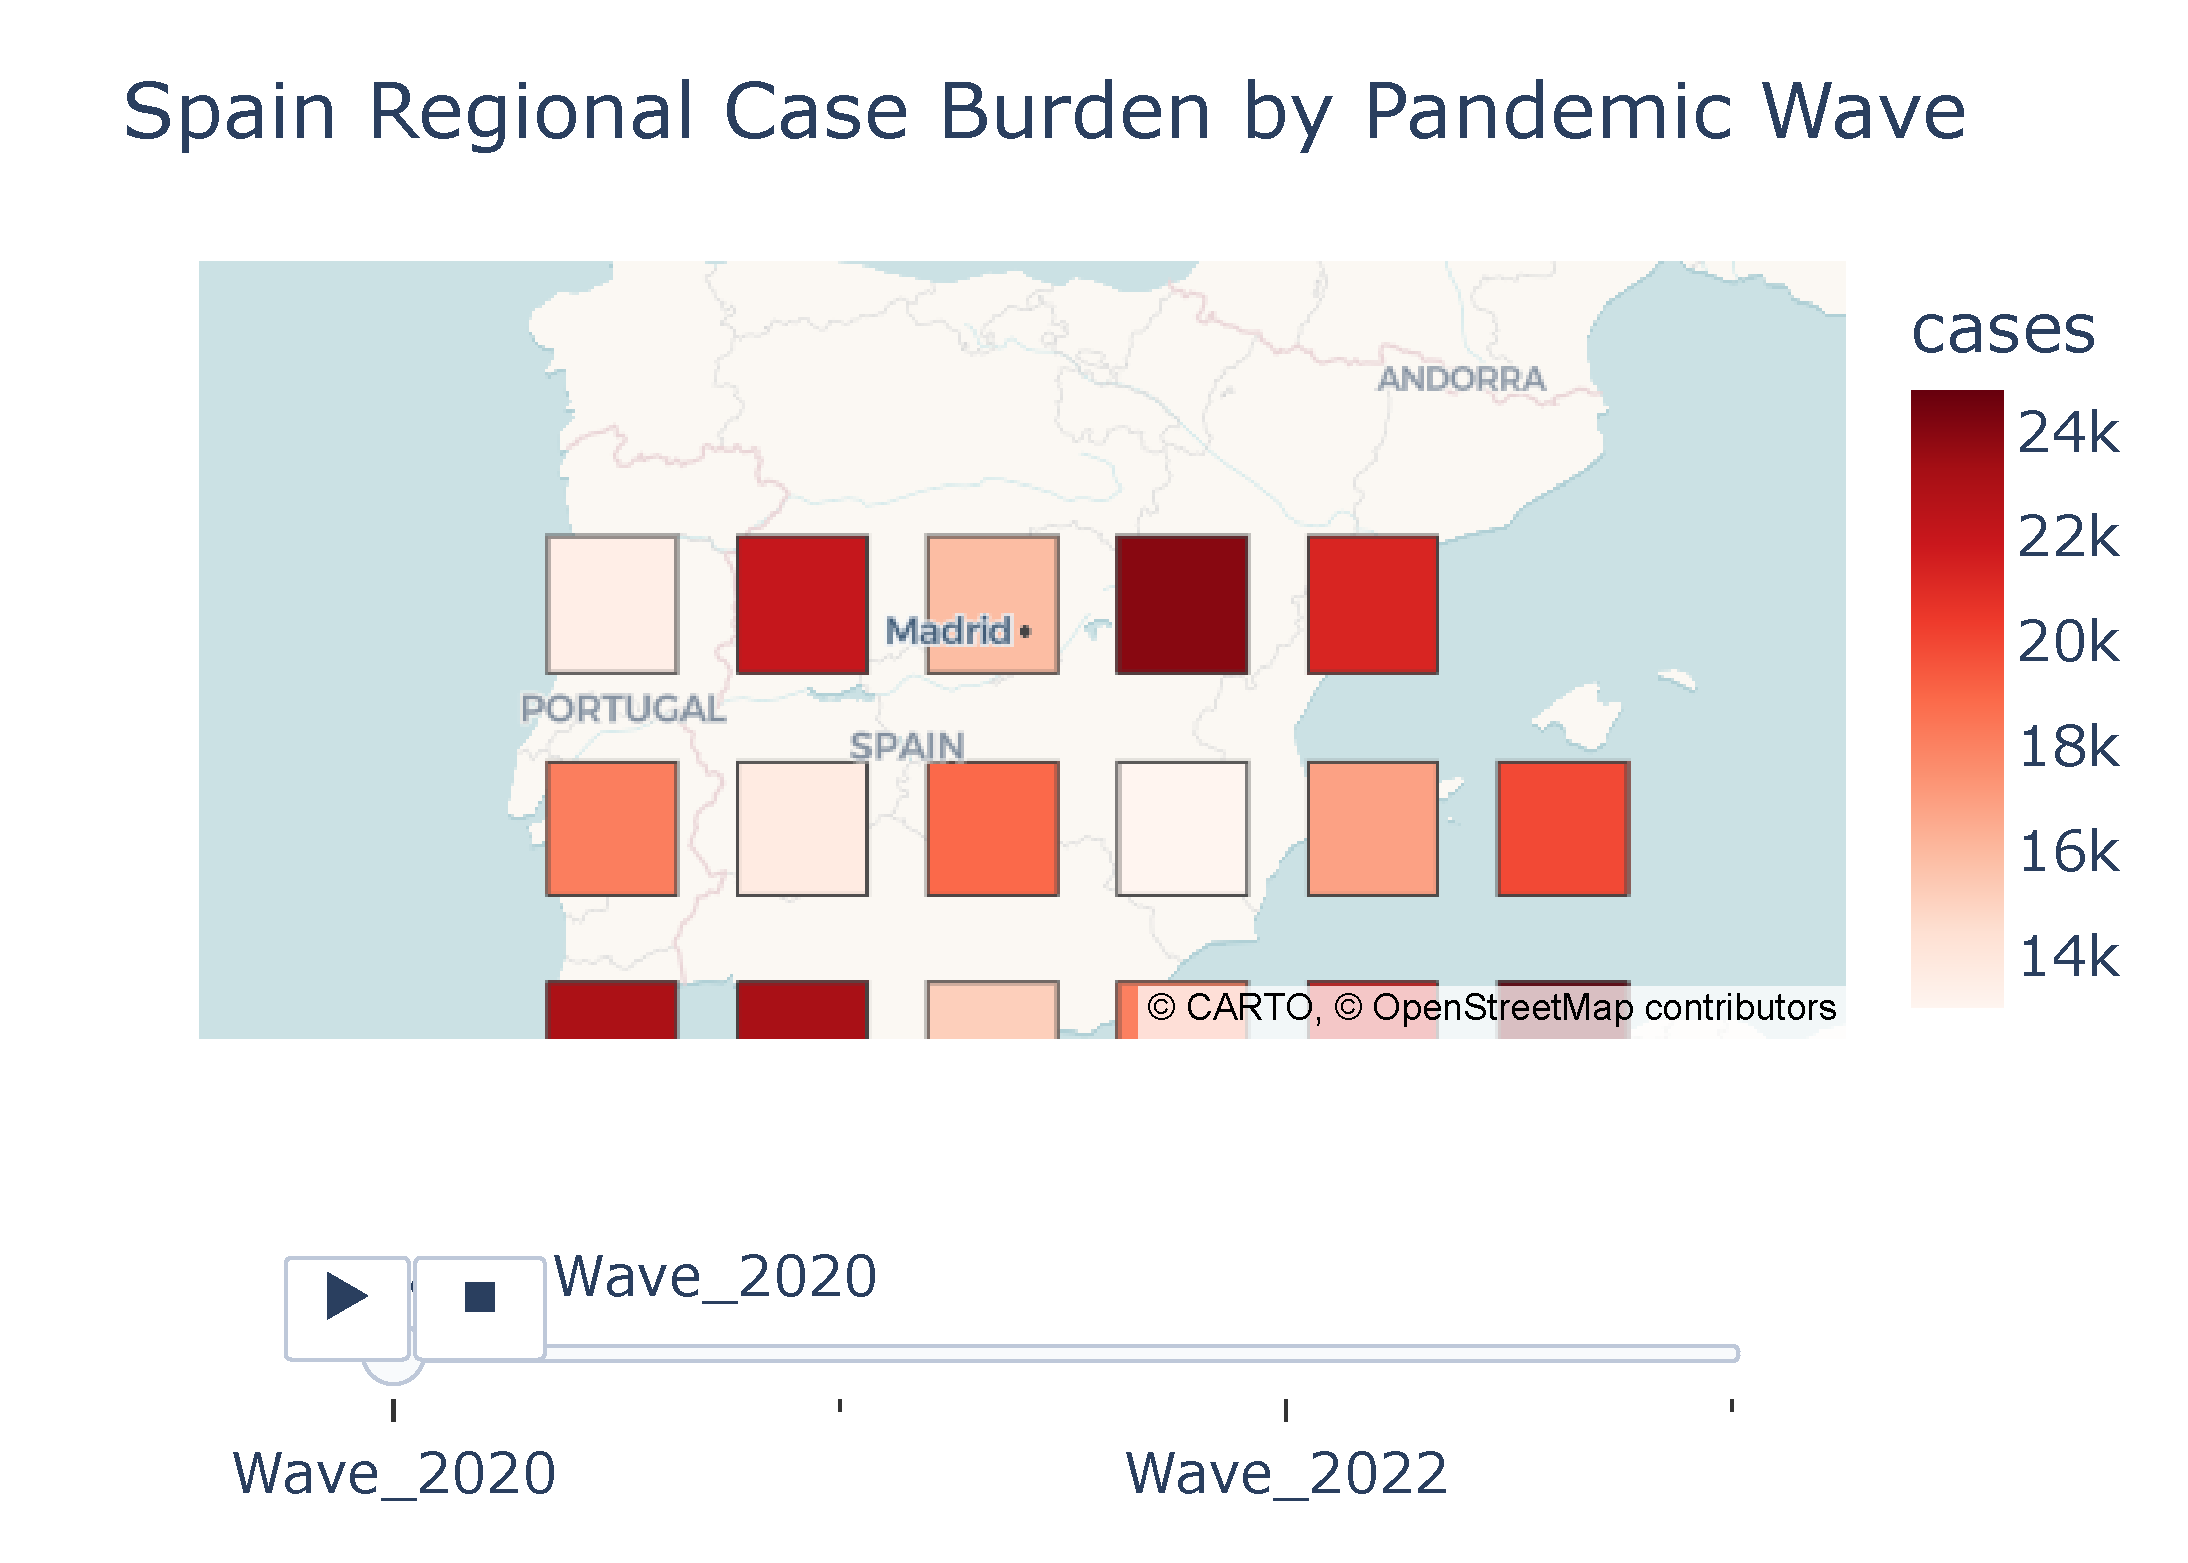
\includegraphics[width=0.95\linewidth]{../figures/static/12_choropleth_waves.pdf}
\end{tikzfigure}

\vspace{0.5em}

\begin{tikzfigure}[Age-sex mortality pyramid. COVID-19 deaths are
  overwhelmingly concentrated in the 70+ age band, with male excess at every
  age above 50 --- a pattern repeated across Europe but especially pronounced
  in Spain due to a high share of nursing-home residents in early 2020.]
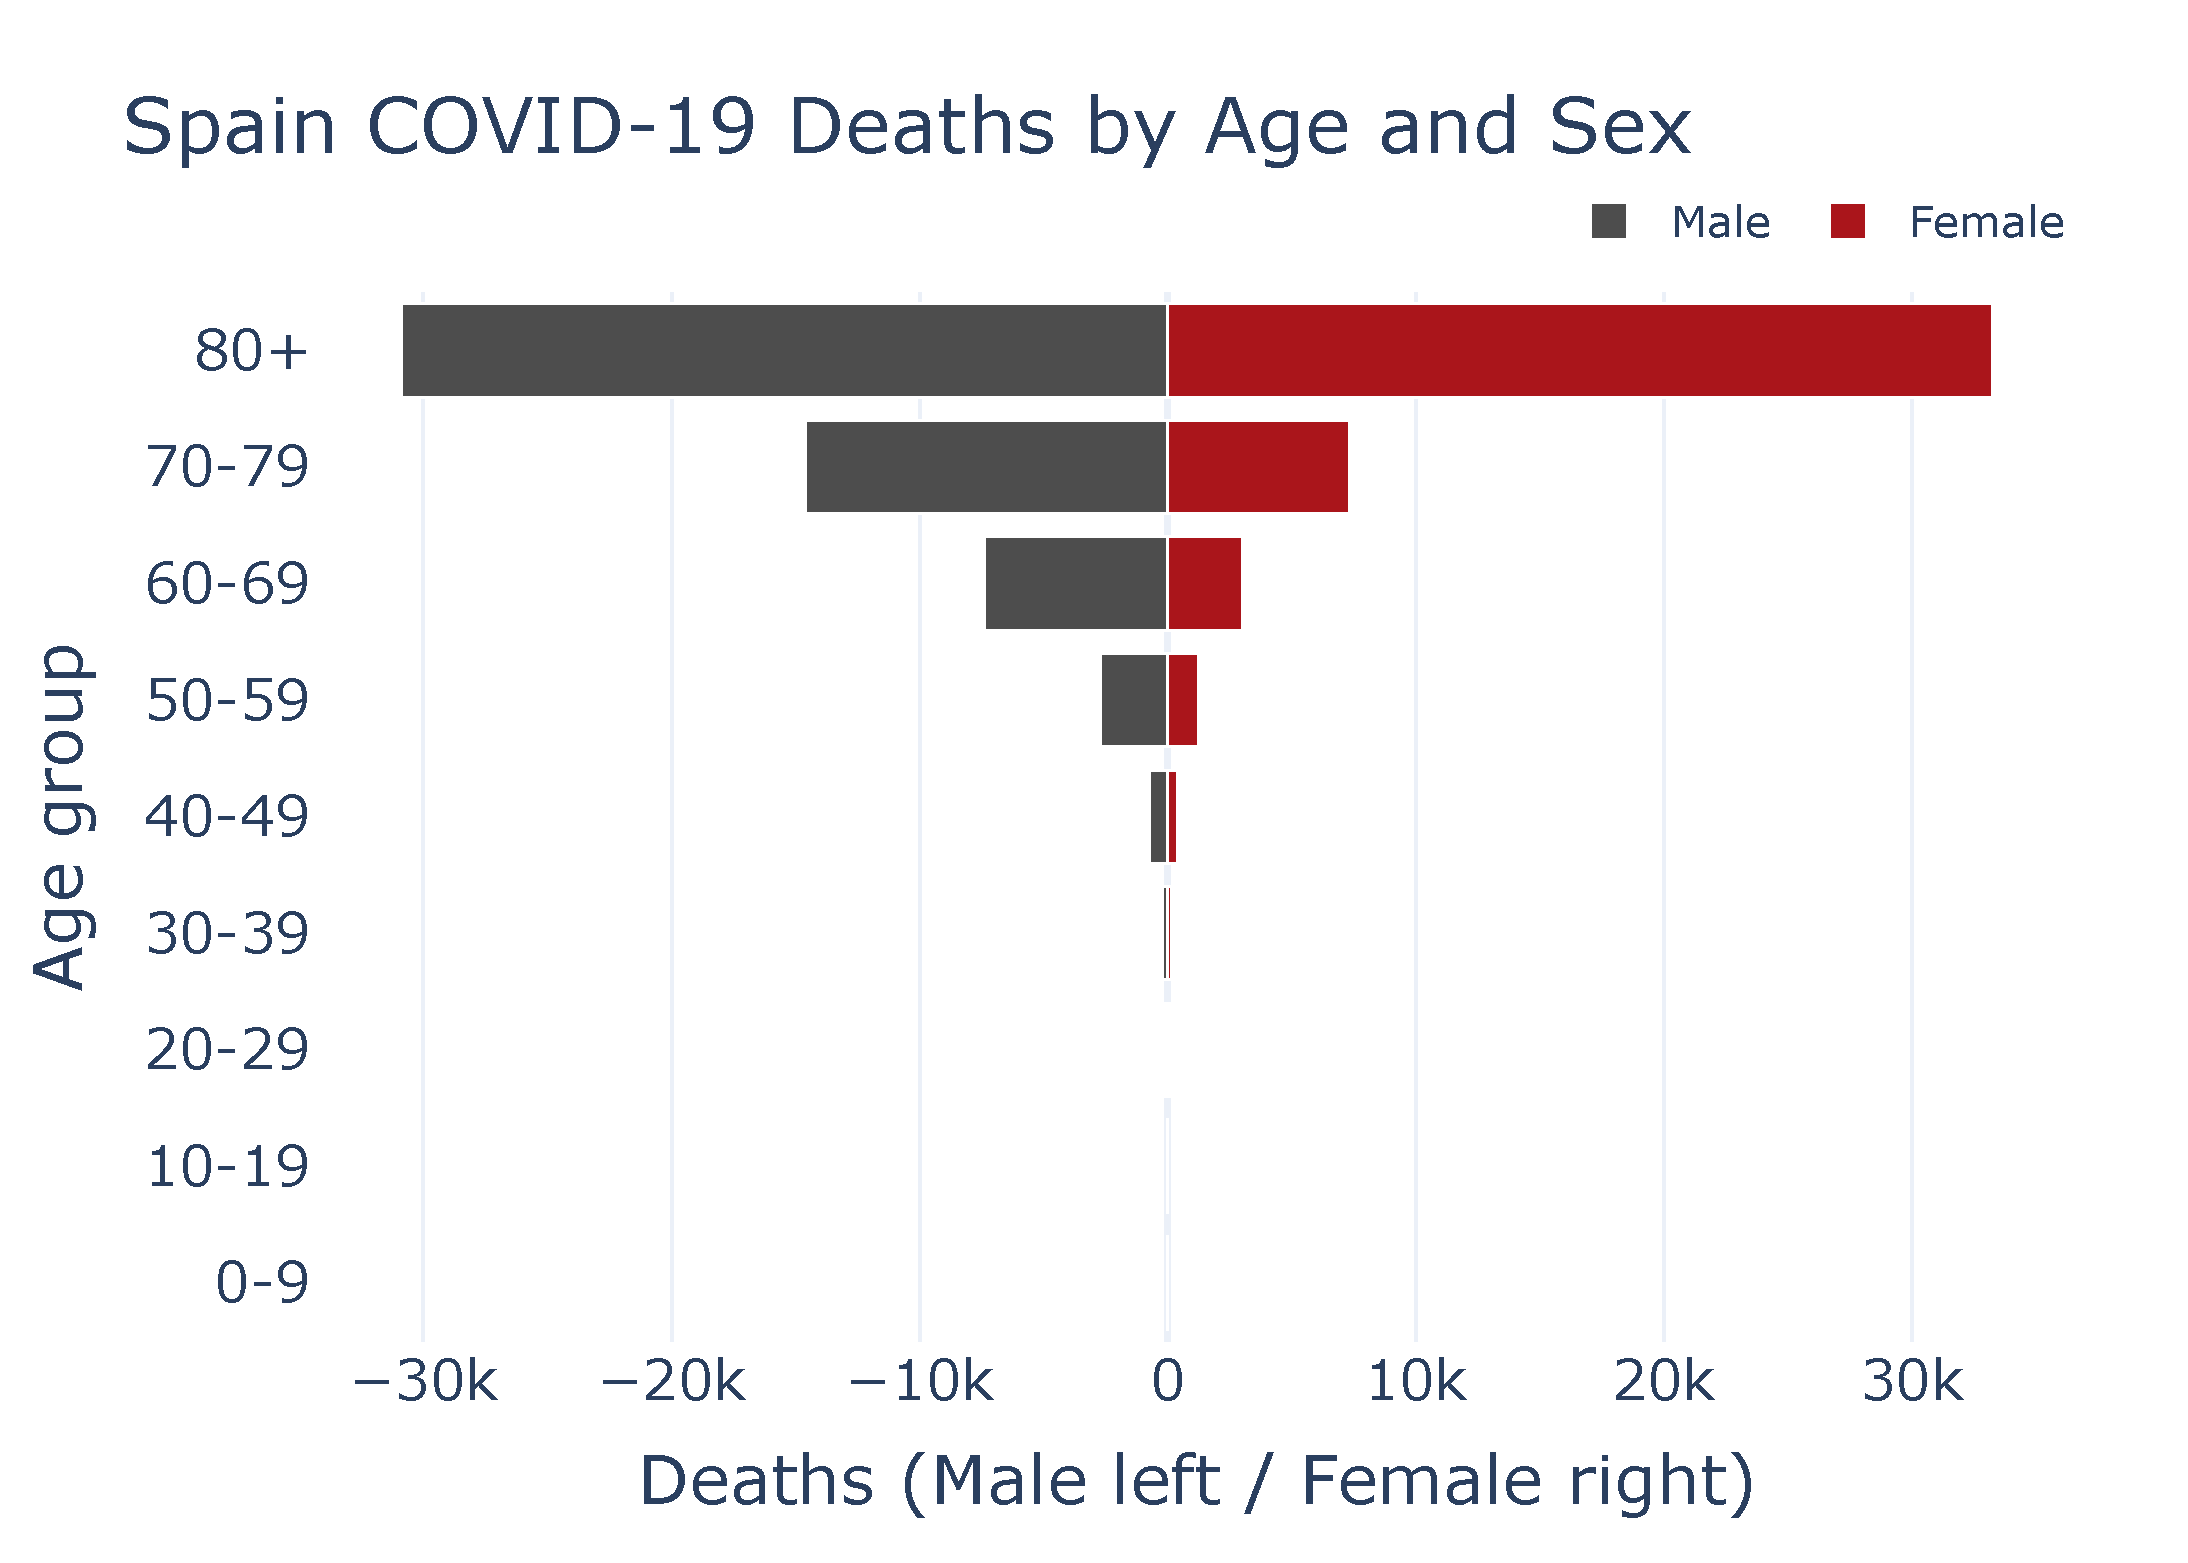
\includegraphics[width=0.95\linewidth]{../figures/static/15_age_sex_pyramid.pdf}
\end{tikzfigure}

\vspace{0.5em}
\large
Spain's burden was \textbf{not} evenly distributed: by region, by age, or by
sex. Public-health planning that treats the country as a single unit misses
where the mortality actually fell.
}

% ── RIGHT COLUMN ─────────────────────────────────────────────────────────────
\column{0.33}

\block{Economy: a tourism shock}{
\begin{tikzfigure}[International tourist arrivals collapsed by 66\% in 2020 ---
  the steepest drop on record. Recovery to pre-pandemic levels took until 2023.]
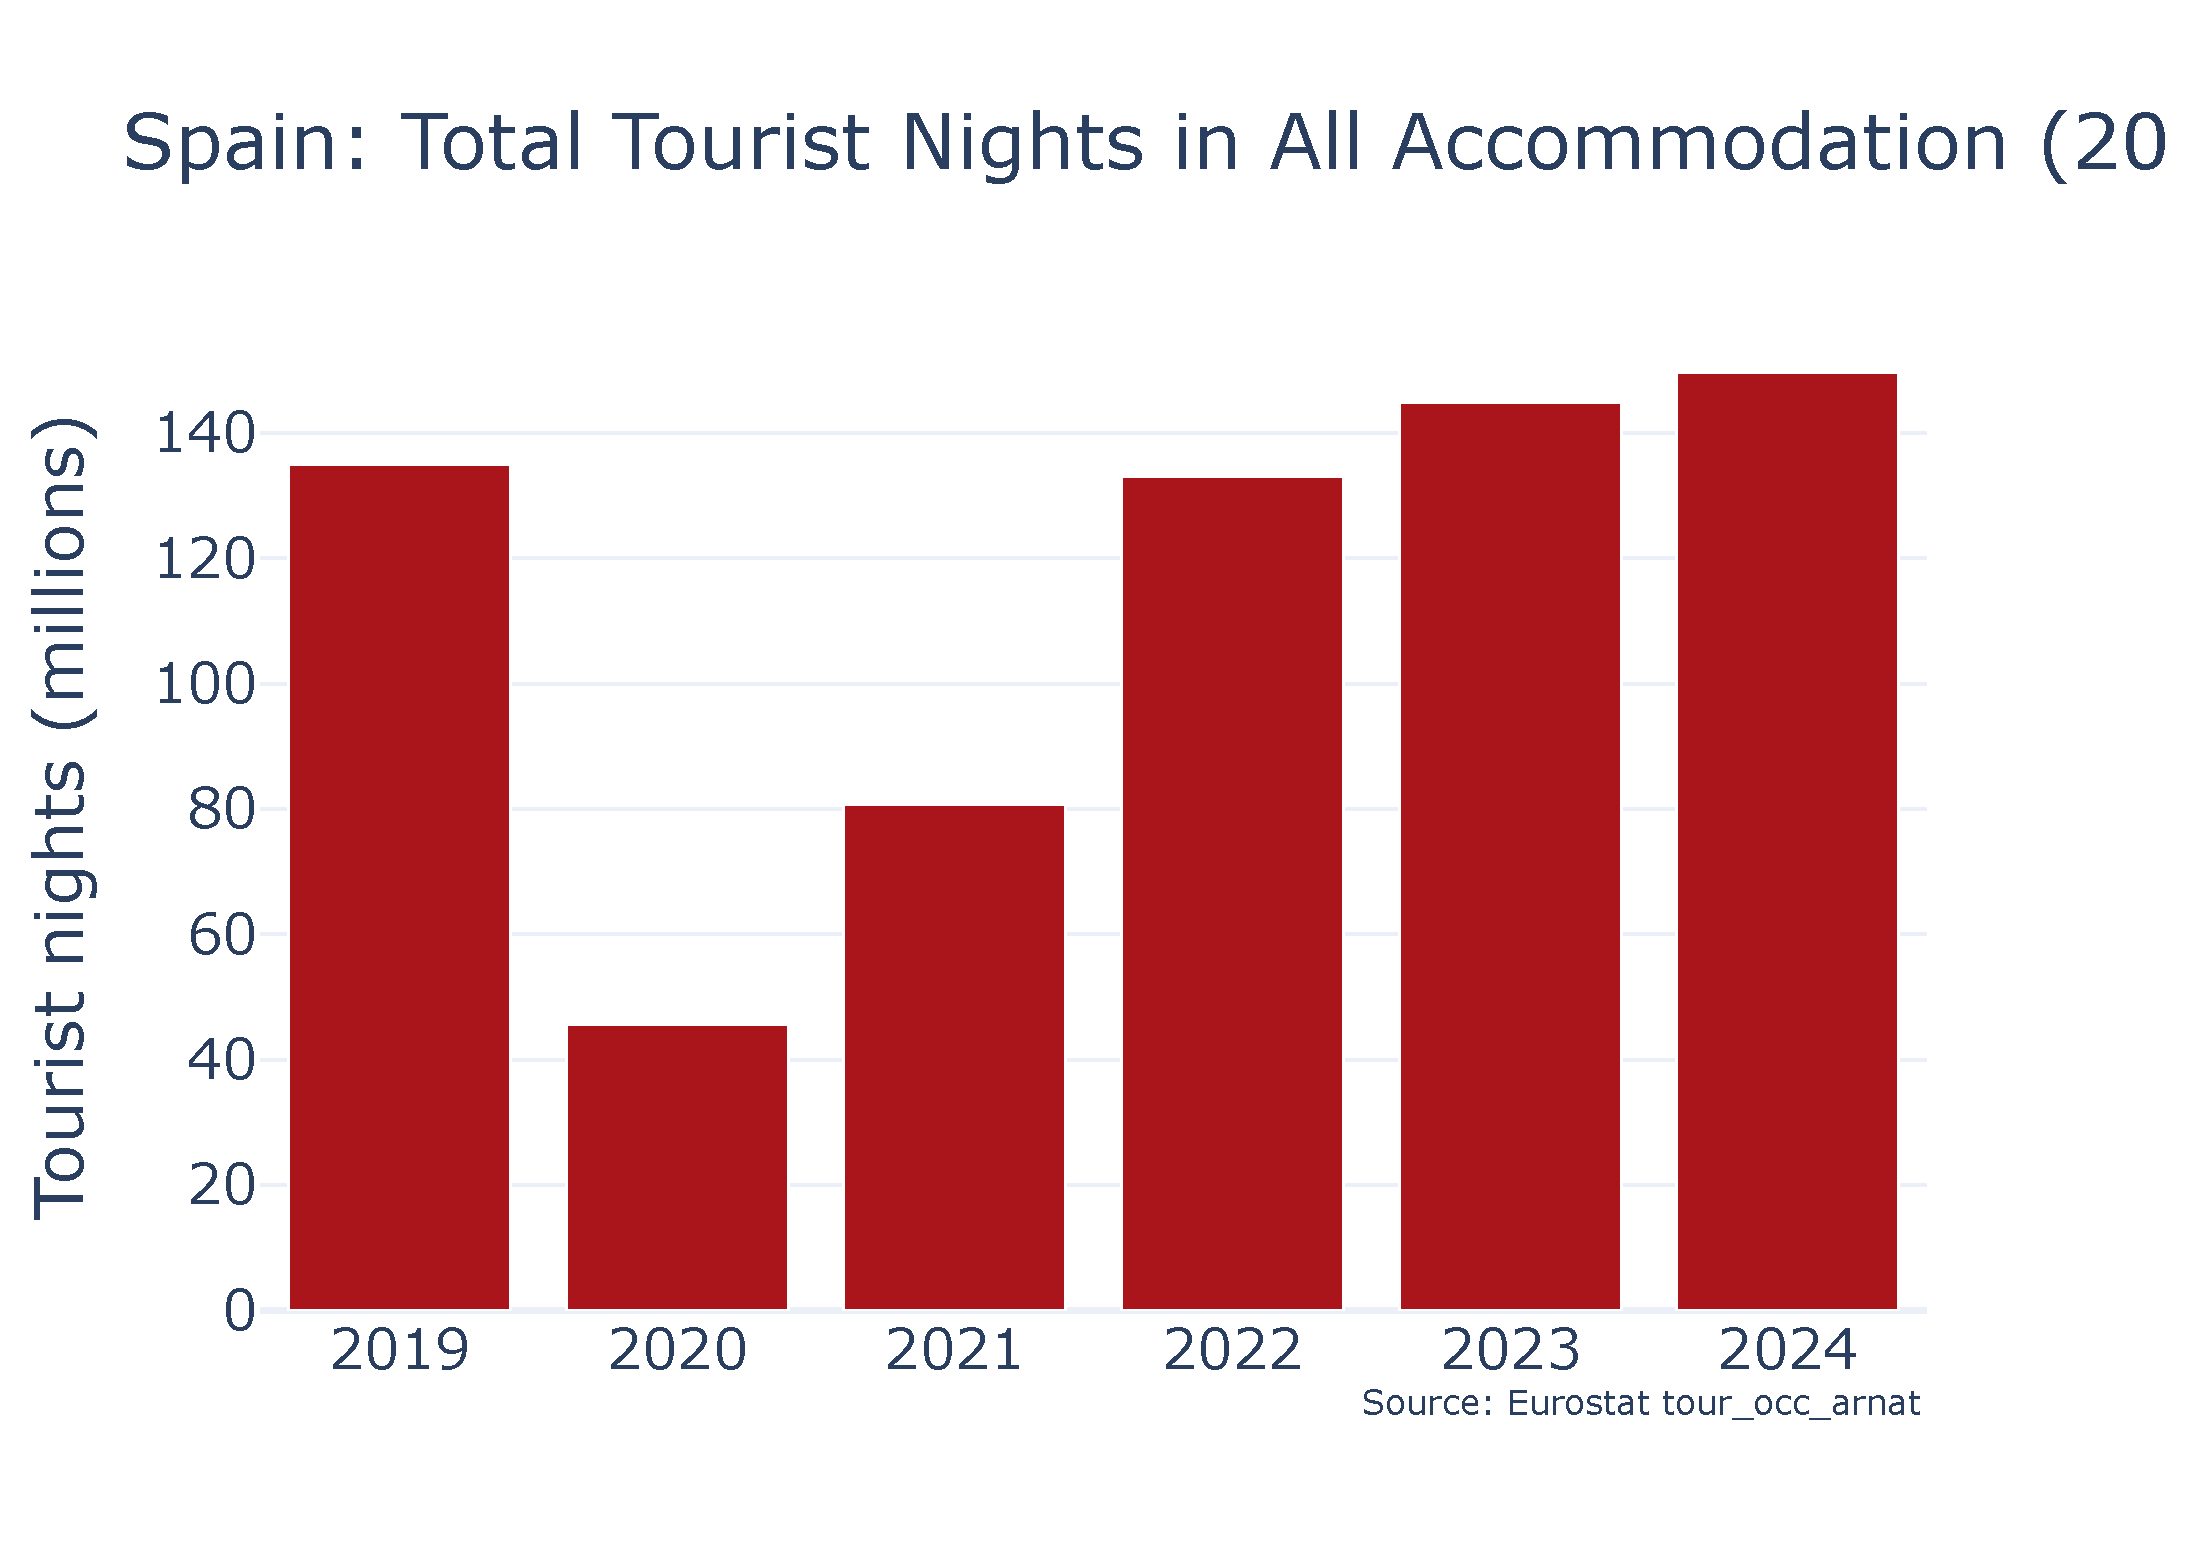
\includegraphics[width=0.95\linewidth]{../figures/static/18_tourism_collapse.pdf}
\end{tikzfigure}

\vspace{0.5em}
\large
Tourism is $\sim$12\% of Spanish GDP. The Balearic and Canary Islands saw
regional GDP contractions above 20\% in 2020 --- the largest of any EU NUTS-2
region. This is the channel through which an epidemiological shock became a
historic economic shock.
}

\block{Inferential: forecasts depend on what you train on}{
\begin{tikzfigure}[Prophet forecast of daily cases. \emph{Top:} model trained
  on 2020--2022 only --- it cannot ``see'' the post-Omicron endemic decline
  and overshoots dramatically. \emph{Bottom:} the same specification trained
  on 2020--2024 produces a plausible flat endemic baseline. Same model, very
  different conclusions. Prophet's logistic growth floor prevents negative
  predictions.]
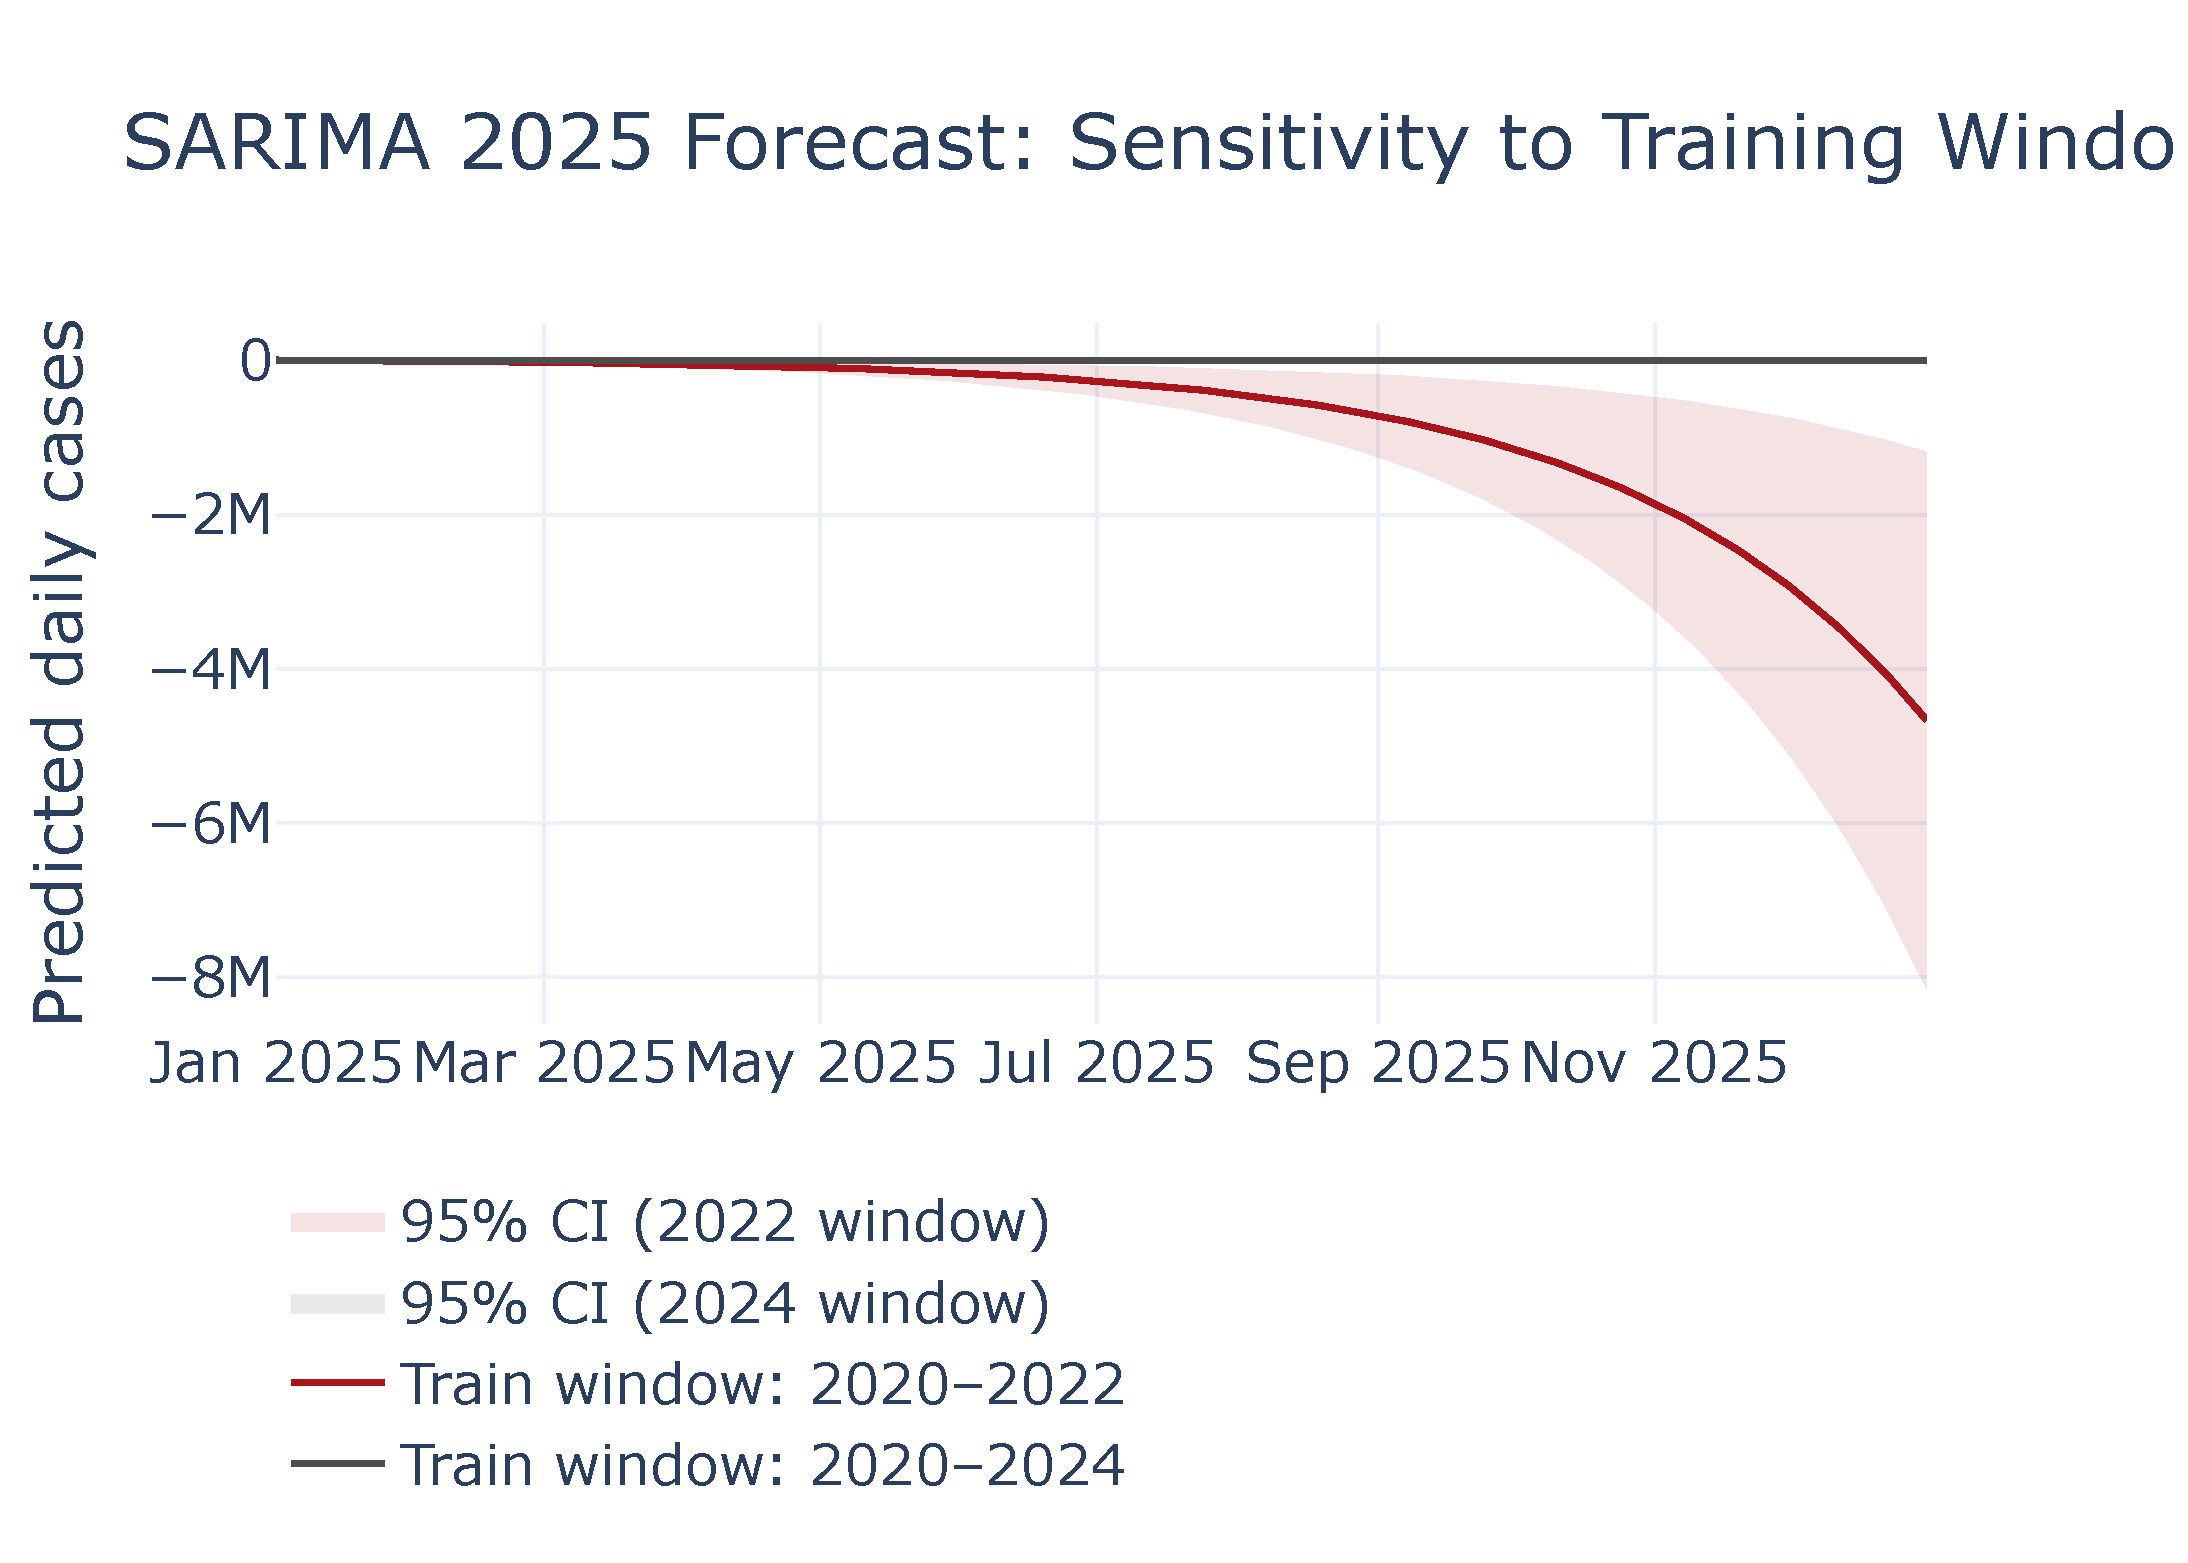
\includegraphics[width=0.95\linewidth]{../figures/static/22_sarima_2020_2024.pdf}
\end{tikzfigure}

\vspace{0.5em}
\large
\textbf{Take-away.} For a disease in transition from epidemic to endemic,
training-window choice dominates model choice. We report both windows
deliberately rather than picking the one that ``looks right''.
}

\block{Conclusions}{
\large
\begin{itemize}
  \item Spain's first wave was among the deadliest in Europe; excess
        mortality shows that confirmed counts \textbf{understate} it sharply.
  \item Mortality is concentrated in the elderly and in inland regions ---
        a national average hides what matters.
  \item The tourism-dependent economy turned an epidemiological shock into a
        record economic contraction (-11\% GDP in 2020).
  \item Vaccination cut the case-fatality rate by more than an order of
        magnitude between waves 3 and 5.
  \item Prophet forecasts are highly sensitive to training-window choice ---
        a methodological caution, not a model failure.
\end{itemize}
}

\end{columns}

\end{document}
